

\section{Background}

\subsection{Large Language Models}
Natural language processing (NLP) has always been an intricate field because of the complexity of human language. The meaning of a message can vary because of homonyms, tone, context, and other factors that affect the message delivered. %These are some challenges that computers face when trying to replicate or learn human text communication and expressions. 
Previous NLP techniques such as Recurrent Neural Network (RNN) could help in understanding a sentence's context in the short term \cite{Sherstinsky_2020}. However, these struggle when trying to understand longer texts. In contrast, the  transformer architecture \cite{vaswani2023attentionneed}, differs from others because it uses self-attention to understand the relationship between words and positions within a sentence. This enables the model to break ambiguities in sentences. The transformer led to the introduction of LLM \cite{naveed2024comprehensiveoverviewlargelanguage}. These models are trained with large amounts of data to replicate human-like patterns or generate text based on statistical relationships between words.
%, and many of these advancements were made possible by transformers \cite{vaswani2023attentionneed}. 

%PreviouHowever, this changed with the introduction of LLM \cite{naveed2024comprehensiveoverviewlargelanguage}. These models are trained with large amounts of data to replicate human-like patterns or generate text based on statistical relationships between words, and many of these advancements were made possible by transformers \cite{vaswani2023attentionneed}. 
%
%Previous NLP techniques such as Recurrent Neural Network (RNN) and Long-Short Term Memory (LSTM) could help in understanding a sentence's context in the short term \cite{Sherstinsky_2020}. However, these struggle when trying to understand longer texts. In contrast, transformer architecture, differs from others because it uses self-attention to understand the relationship between words and positions within a sentence. This enables the model to break ambiguities in sentences. 

\subsubsection{LLM Architectures}
LLM have different architectures, designed for performing specific tasks:

\begin{itemize}
\item{\textbf{Encoder-only models:}} These models are like BERT \cite{DBLP:journals/corr/abs-1810-04805}. This type of model predicts text by masking specific words in a sentence. They are better for classification and sentiment analysis.
\item{\textbf{Decoder-only models:}} These models include the well known GPT-3 \cite{DBLP:journals/corr/abs-2005-14165}. They receive one input and try to predict the entire text. They are good for summarization and text-generation.
\item{\textbf{Encoder-Decoder models:}} An example is T5 \cite{2020t5}. These mask entire sequences of text, and are good for translation and question  answering.
\end{itemize}

%\begin{figure}[htbp]
%    \centering
%        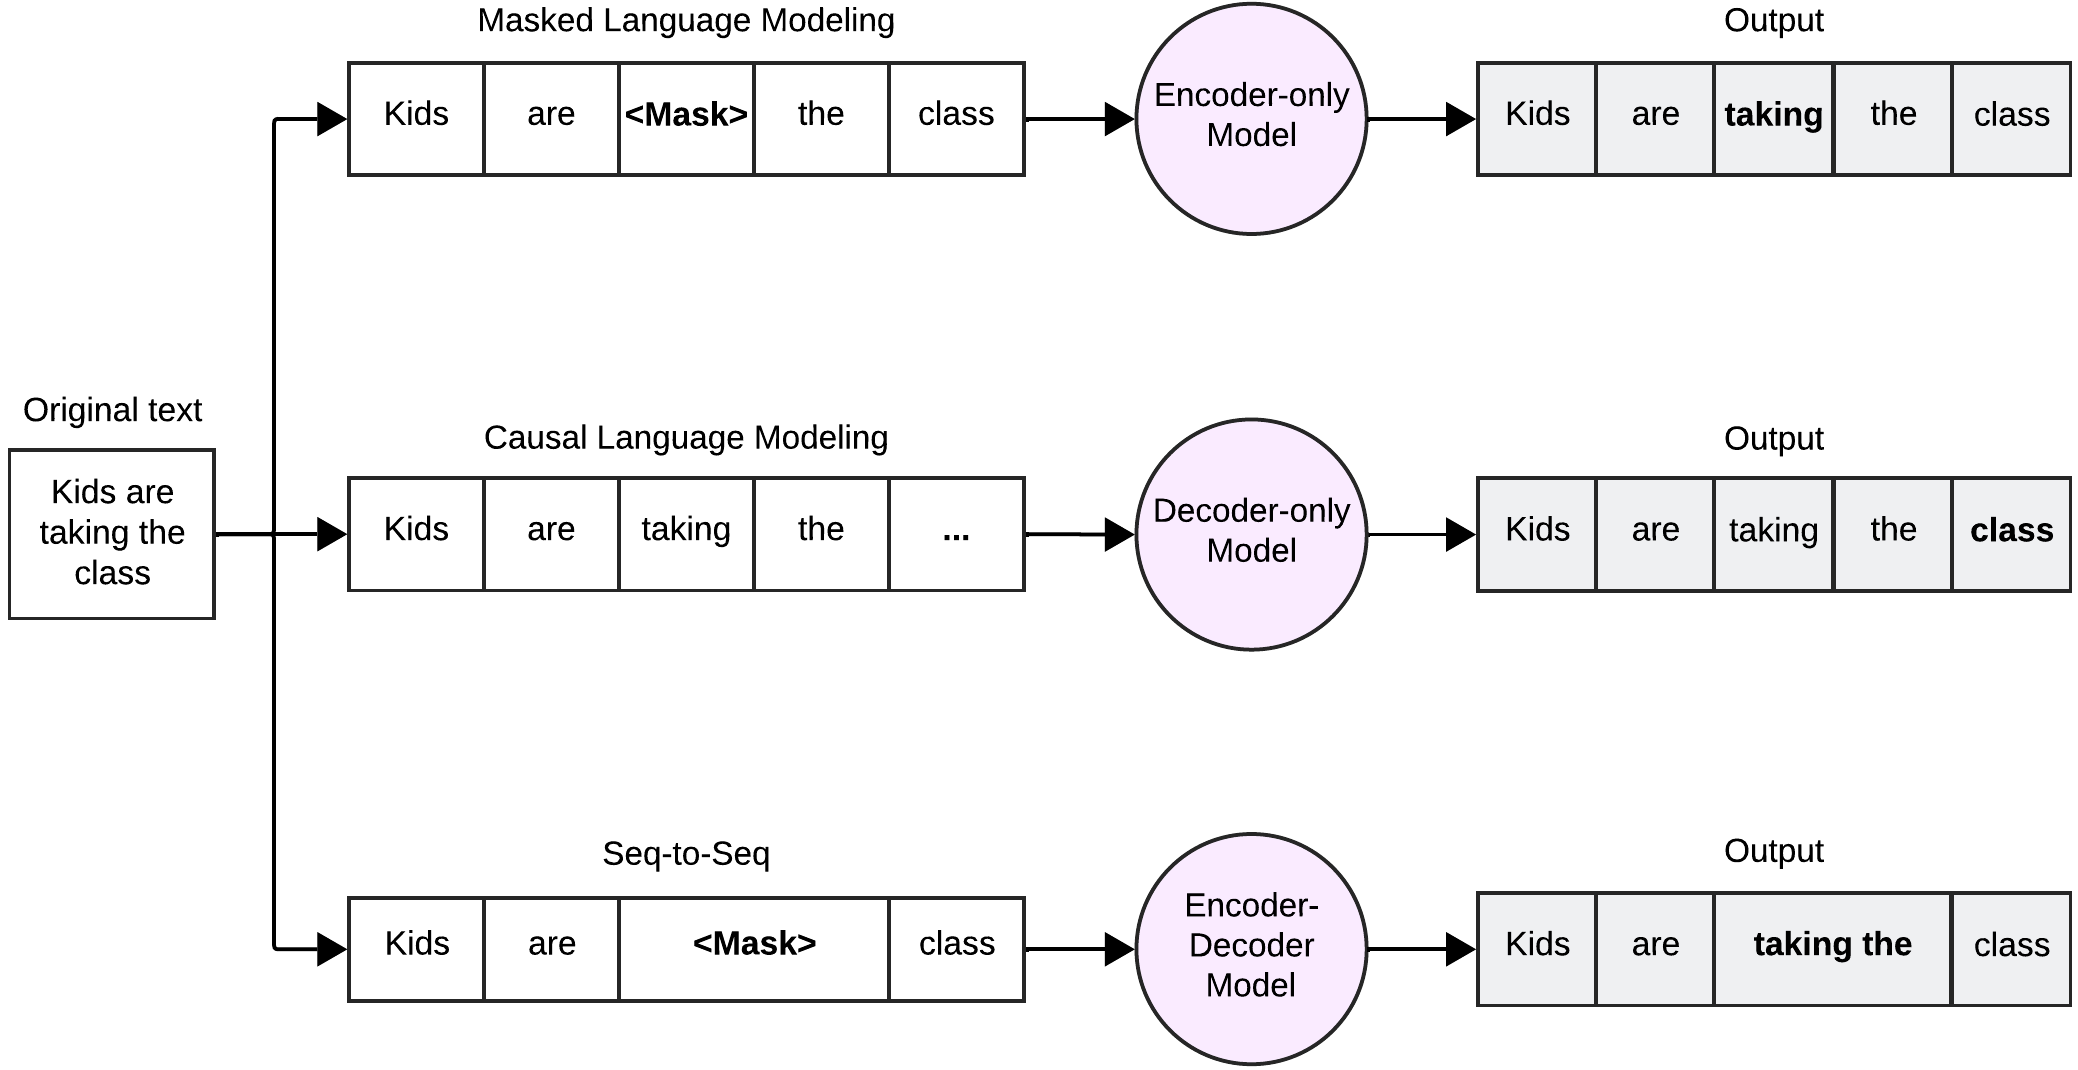
\includegraphics[width=0.5\textwidth]{figures/LLM_Arch_text_generation.png}
%        \caption{The transformer architecture}
%        \label{architecture}
%\end{figure}


%\subsubsection{Example Applications}
%The authors in \cite{koh2023groundinglanguagemodelsimages} trained a based LLM model to understand images and give a text description or a combination of text and image. The training process for
%the model used images and their captions as their data and the zero-shot learning strategy. Their resulting model was used as a chatbot that identifies images, answers questions, or gives
%visual examples. Another experiment was \cite{inproceedings}, where the authors trained a model to identify sentiments on financial market decisions. In this case, they used prompting, also called in-context learning, for 
%the model to answer the sentiment of the texts. In-context learning does not update any parameter of the original model. Their model resulted in a 70\% accuracy on sentiment prediction, failing mostly on neutral posts.
%That experiment showed the problem that users face when they use social media to make decisions. They clarified the importance of not taking the model for granted and how social media can cause a user to make a poor decision.

\subsubsection{Challenges and Limitations}
An issue with LLM is that they answer based on statistical relationships between words, and occasionally, their output could make no sense. They could generate a result that is not factual
or valid; this phenomenon is called an {\em hallucination}. Without additional context, they cannot differentiate between fact and fallacy. %This context needs to be similar to the input that the model
%receives. 
%However, finding the necessary information is not optimal if done manually.

\subsection{Vector Databases}
We can reduce the hallucinations by providing textual context relating to the input text (e.g., premise). A solution to this is finding data from official, curated sources  on the topic associated with the premise text. That data can be stored
in a vector database, which stores text data in a multi-dimensional vector representation.  Some database  engines support vector searches natively, like Chroma \cite{chroma}, while others have extensions,
like Postgres with its pgvector  module \cite{pgvector}. These vector databases turn images, documents, and others data into numerical vectors known as {\em embeddings}. These embeddings are numerical vectors capturing semantic meaning \cite{10455990}.
 
When querying the database, it will return text chunks that can function as context for an LLM to analyze. This becomes additional input that the LLM can use to generate an answer. Thus, an LLM can use the retrieved chunks to generate a fact-checked answer. % from outside their initial training.
 The work in \cite{10683437}  tested LLM to answer a question that contained images and text. They evaluate the GPT3 base model, the base model with prompt engineering,
and a GPT3 with RAG. Their experiments showed that the base model's average success ratio was 40\%, the second model was 58\%, and the model with RAG ended with 75\%. Said experiment illustrates  that
an LLM can have high performance when it receives the necessary context. 
%Therefore, RAG can assist in providing expert-level responses.%, but human oversight is still imperative for complex topics. 
%Additionally,
%in a world with many sources of information that can be misleading to people, this can help identify texts that are not factual. 

\subsection{Misinformation in Social Media}
%There are many sources in the world to find information about any topic. Nonetheless, many people use social media as their primary source \cite{socialmedias} and occasionally take this information as truth without
%validation \cite{social_fact}. On occasion, these can be fake or misleading. When this happens unintentionally or by lack of understanding of the topic, it is called misinformation. On the other hand,
%when it is intentional to provide wrong information, this is known as disinformation. For simplification, both terms will be used interchangeably, as they have a similar impact on the user, by providing inaccurate information.

Misinformation has been dangerous during critical events like natural disasters or health crises. For instance, during the COVID-19 pandemic, false claims appeared saying that the vaccine had
microchips or that it was intended for population control \cite{article_vaccine}, which led to high health risks or even deaths \cite{article} because people refused to get vaccinated out of fear. 
%A problem with disinformation is that the audience
%does not always detect it. When misinformation spreads and is not clarified early on, it can be confused as fact. Misinformation can affect all demographics, but older audiences and people with less education are more
%likely to share and believe misleading news \cite{encyclopedia3040099}. 

There have been various research studies on reducing the propagation of misinformation. Misinformation was modeled as a game-theoretic problem in \cite{9906925}, where some players spread fake news, and others tried
to stop it. They created an agent at the network level to combat misinformation in a simulation. However, they could not conclude the efficiency of their model due to the lack of discernible patterns in the simulation. On
the other hand, the authors in \cite{10100054} used LSTM and BERT to classify misinformation from the different news sources. They showed that BERT outperformed LSTM, achieving an accuracy of 64.88\% against 60.59\%. 
%These results are significant in detecting misinformation; still, they are not optimal for situations that can directly impact someone's life. For example, the system has over a third chance of misclassifying news, and this could
%be dangerous if the topic is a natural disaster or health risk. We need to ensure that AI models classify this type of news with a very high accuracy rate. These researches showed the efficiency of LLM in the misinformation field.
%Regardless, they do not address health-related misinformation on social media. 

%Another approach to detecting fake information was on \cite{Ayoobi_2023}, where they detected fake LinkedIn profiles. On this occasion, the dataset used for training included real and AI-generated profiles. They tested multiple
%LLMs like BERT and RoBERTa, but BERT resulted in the highest accuracy of 95.67\%. These researches showed the efficiency of LLM in the misinformation field. Regardless, none of them addresses health-related misinformation on social media. 

When combatting misinformation, the difficulty arises when determining what is spreading and how experts can correct it. It requires  credible sources or an expert on the field, to verify the truth.
%Some disinformation can be easier to identify such as hoaxes, but other things, such as conspiracy theories, require more resources to debunk. 
These tasks are time-consuming and the rebuttal
%to refute it the
%explanation 
must be expressed so that any audience can understand it. 
%These are a few reasons that health-related misinformation is hard to combat.
 %Experts in the field must be fast at identifying the 
%misinformation and concise when correcting it. 
LLM can combat misinformation by classifying it and rebutting it. 
%For the classification process, it is possible to
%fine-tune an LLM that determines if a text has misinformation. Additionally, it can generate rebuttals using RAG. With a vector database that contains peer-reviewed research, it can ensure that the information is factual. 
This AI approach can reduce the dependency on experts and have a system that can act in real-time to mitigate misinformation.


\subsection{Twitter Health Surveillance (THS)}
The THS system classified tweets related to health issues \cite{8622504, 9581175}. The system utilized LSTM and GRU to classify tweets as being medical related, unrelated, or ambiguous.  The THS
data extraction pipeline can be found on Figure \ref{ths_architecture}. THS extracted data from the Twitter API and processed it through the Apache ecosystem. Later, a preprocessing phase
for each tweet occurred, which removed hashtags, mentions, emojis, and web links. The classification agent trained with the resulting plain text. This version used recurrent neural network (RNN) and
1-d convolutional neural networks (CNN) because of their advantages with sequential data. The authors tested various  architectures, and the one with the highest result was an LSTM layer (with no attention) followed by a
and a GRU layer.  
%T had an F1 score of 86\%, a recall of 89\%, and a precision of 83\%.   
However, these experiments removed special elements from the original text,  %By then, tweets had a limitation of characters, making each one of the crucial. 
%Removing special characters, 
which could remove valuable insights. 
% that the author of the text intended. 

 
  \begin{figure}[!h]
    \centering
        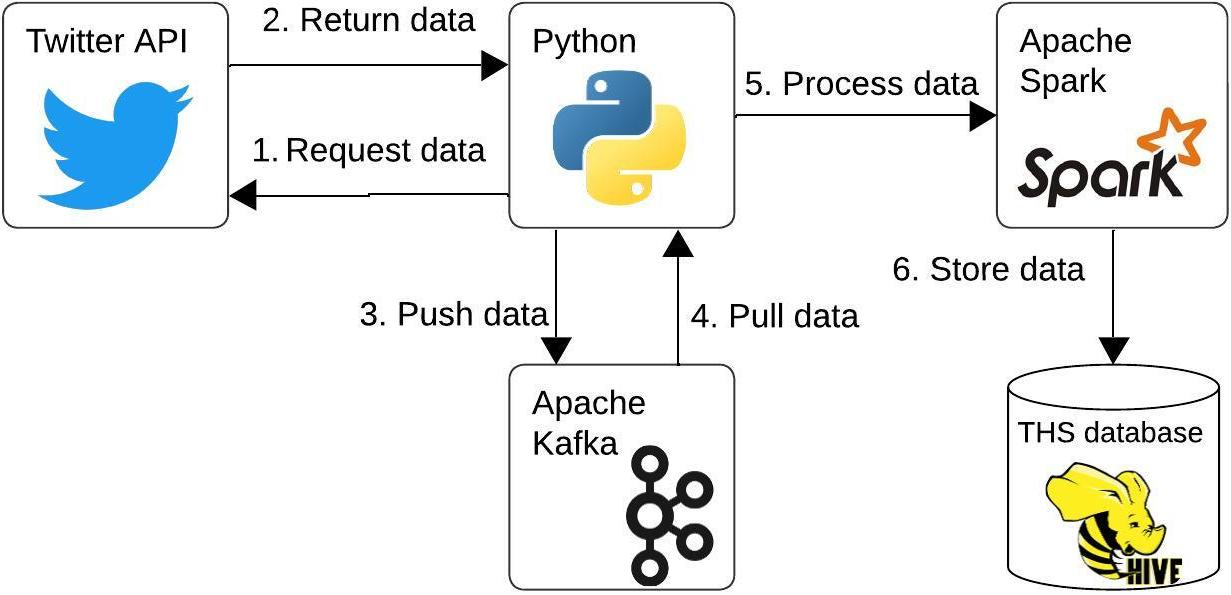
\includegraphics[width=0.42\textwidth]{figures/ths_architecture.jpeg}
        \caption{THS Architecture}
        \label{ths_architecture}
\end{figure}

%Later the project was updated to find similarities between tweets \cite{9581175}. This new version tested CNN and RNN to classify how closely related are two different tweets.
%They used a ranking method that gave a higher score if two randomly selected tweets were similar. The agent received an input of triplets where the first element was compared against the other two elements.
%The system trained on two data types: raw tweets and cleaned tweets. This latter had stop-words removed and a lemmatization process. Cleaned tweets proved a higher accuracy in the RNN
%for regular LSTM and bidirectional networks; in contrast, the raw tweet had a better result in CNN validation. All three models had similar results; the highest validation accuracy was the regular LSTM with 90\%,
%followed by the other two with 87\%. Nonetheless, the training time for the CNN was the fastest, with regular LSTM in second place and the slowest being the bidirectional LSTM network. 

%However, both of these experiments removed special elements from the original text. By then, tweets had a limitation of characters, making each one of the crucial. Removing special
%characters, could remove information that the author of the text intended. 


%
%\subsection{Large Language Models (LLM)}
%
%The are three different architectures for Large Language Models, encoder-only, decoder-only, and encoder-decoder. Each one has advantages on specific tasks. In Figure \ref{architecture}
%
%\subsubsection{Encoder-only models}
%These models are like BERT.
%This type of model predict by masking specific words in a sentence.
%They are better for classification and sentiment analysis.
%
%\subsubsection{Decoder-only models}
%For these model we have the well known GPT-3.
%They receive one input and try to predict the entire text.
%They are good for summarizing and text-generation.
%
%\subsubsection{Encoder-Decoder models}
%T5 is an encoder-decoder models.
%They mask entire sequences of text.
%Good for translation and question and answering.
%
%\begin{figure}[!ht]
%    \centering
%        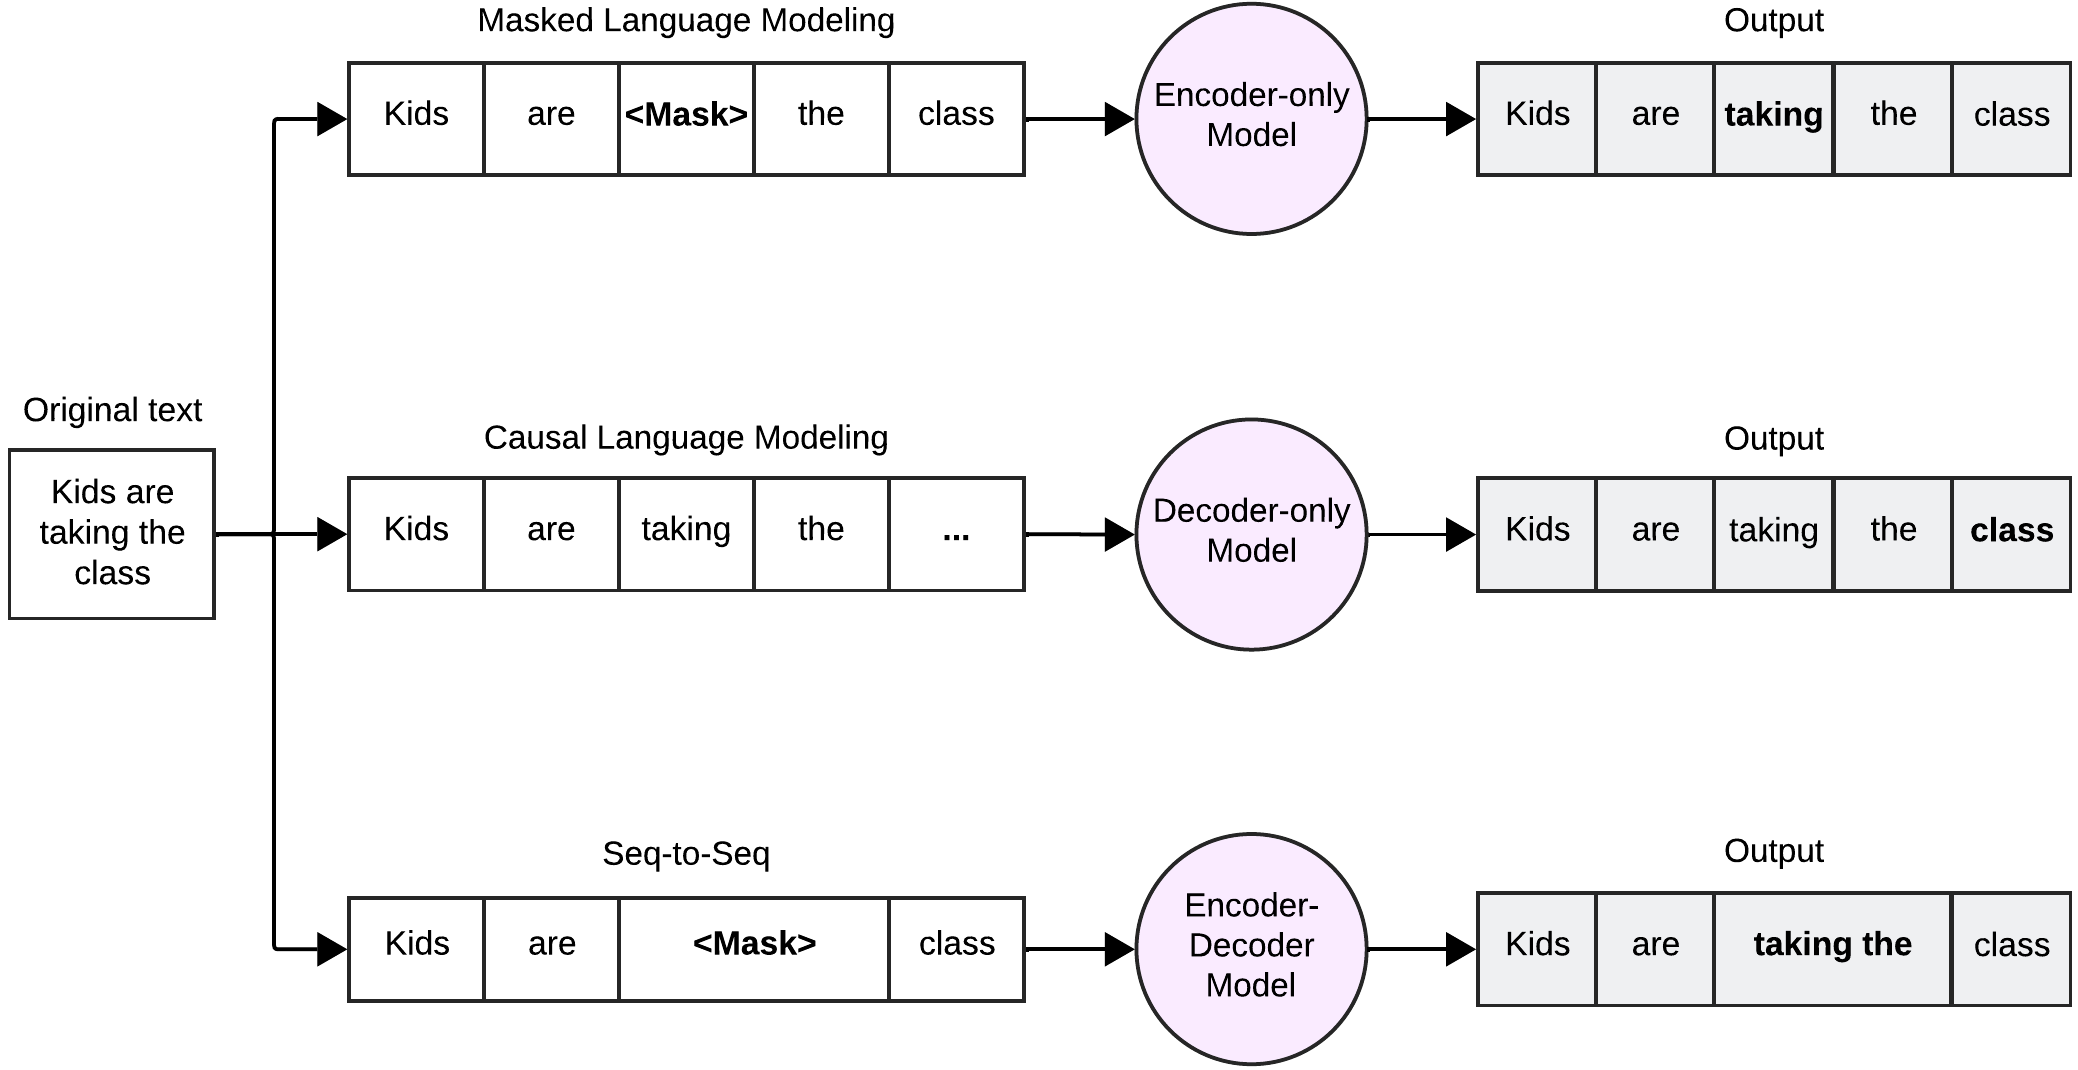
\includegraphics[width=0.5\textwidth]{figures/LLM_Arch_text_generation.png}
%        \caption{The transformer architecture}
%        \label{architecture}
%\end{figure}

